% !TeX root = ../main.tex
\chapter{Methods}

In this chapter, we will talk about the experiments conducted in this study, including the experiment designs, data processing, analyses, results, and discussions. The first experiment is a production task that measures both carry-over and anticipatory effects in Taiwan Mandarin and Taiwan Southern Min. The second experiment is a replication of \cite{Zhangetal2022}, where the magnitude of normalization of tonal coarticulation is measured. The last is a word-non-word test, aiming to examine the subjects strictness on tone boundaries.


\section{Experiment 1}
Experiment 1 measures tone productions in monosyllabic and disyllabic words in Taiwan Mandarin and Taiwan Southern Min. This experiment seeks to reexamine the magnitudes and behaviors of tonal coarticulations in these two languages.

While it is established in the literature that the pitch values of Mandarin tones are subject to those of their preceding (carry-over effects) and following tones (anticipatory effects), with carry-over effects being stronger and assimilatory, and anticipatory effects being weaker and generally dissimilatory, studies on tonal coarticulation in (Taiwan) Southern Min lead to less consistent results: while \cite{Peng1997} found anticipatory tonal coarticulation in Taiwan Southern Min, and \cite{Wang2002} stronger carry-over effects and weaker anticipatory effects, \cite{ChangHsieh2012} found inconsistent assimilatory and dissimilatory effects for both carry-over and anticipatory coarticulations. This might be due to the different experiment designs and dialects examined: in \cite{Wang2002}, non-words were used as stimuli, with syllables also found in Taiwan Mandarin. Such design might have led the speakers to be influenced by Mandarin, in which they were presumably also native; in \cite{ChangHsieh2012}, it was Malaysian Hokkien that was examined, while in \cite{Peng1997} and \cite{Wang2002}, it was Taiwan Southern Min. A reexamination with a consistent design is thus in need if we are to compare tonal coarticulations in these two languages, and to observe how the differences in tonal coarticulations may exert different effects on the way the speakers of the two languages normalize for them perceptually.

\subsection{Participants}

This study recruited 43 Taiwanese college students as participants (25 females; 20–27 y.o., mean=21.93). 15 of them were native speakers of Taiwan Mandarin. These subjects were not speakers of Taiwan Southern Min (upon self-report). These speakers are hereafter refereed to as the monolingual group. 28 of them were native speakers of Taiwan Southern Min. These subjects were also speakers of Taiwan Mandarin. These speakers will be referred to as the bilingual group. Among the bilingual speakers, 11 speakers were advanced Taiwan Southern Min speakers, with self-reported points of 8 or higher on a fluency scale from 1–10. These 11 speakers will be referred to as the advanced bilingual group. The rest of the bilingual speakers will be referred to as the intermediate bilingual group. All of the subjects were not speakers of other tonal languages. See Appendix \ref{Appendix:ParticipantInfo} for a full list of the participants. 

For Experiment 1, only the monolingual speakers\footnote{Except for P22, who only participated in Experiments 2 and 3.} and the advanced bilingual speakers participated. The monolingual speakers produced the Mandarin stimuli; the bilingual speakers produced both the Southern Min and Mandarin stimuli.

\subsection{Stimuli}
To examine the influence of ambient tones on the target tones, a disyllabic word was chosen for each of the 16 (4 tones × 4 tones, for Taiwan Mandarin)/25 (5 tones × 5 tones\footnotemark, for Taiwan Southern Min) tone combinations as stimuli. Syllables with voiceless obstruents, affricates or fricatives were avoided. In addition, to observe the tones in neutral positions , 4 monosyllabic words with the 4 tones were chosen for Taiwan Mandarin group, and 7 monosyllabic words likewise for Taiwan Southern Min group. These resulted in a total of 20 words for Taiwan Mandarin group and 32 words for Taiwan Southern Min group, with 10 repetitions each. See Appendix \ref{Appendix:StimuliforExperiment1} for a full list of the stimuli.

\footnotetext{Check tones were excluded.}

\subsection{Apparatus}
The audio data were collected with a microphone (Audio–Technica Carcoid AT2035) plus a portable audio interface (USBPre 2), and saved as WAV files, with a sampling frequency of 44100 Hz.

\subsection{Procedure}
Subjects were first led through a list of the stimuli which they would encounter, and made sure they were familiar with the words. The stimuli were then randomly presented on a MacBook Pro (13-inch, 2018) one at a time. For Taiwan Mandarin group, stimuli were presented in traditional Chinese characters; for Taiwan Southern Min group, stimuli were presented in both traditional Chinese characters and romanized forms, with their Mandarin glosses underneath. Subjects were asked to say the word when they saw it, at a relaxed pace. Subjects might press the button and proceed to the next word when they were ready. The stimuli were divided into two blocks in the Taiwan Mandarin version and six blocks in the Taiwan Southern Min version, with a break in between. The whole process would take about 10 minutes for Taiwan Mandarin group and 30 minutes for Taiwan Southern Min group. This experiment was done after Experiments 2 and 3.

\subsection{Data processing}
\subsubsection{Labeling}
The audio data were examined and processed with \textit{Praat} \citep{BoersmaWeenink2018}. Syllable boundaries were labeled and saved as \textit{Praat}’s TextGrid. Boundaries are determined with intensity and formant transition. A part of the TextGrids is shown below in Figure \ref{Figure:TextGridExample}.

\begin{figure}[hbt!]
\centering
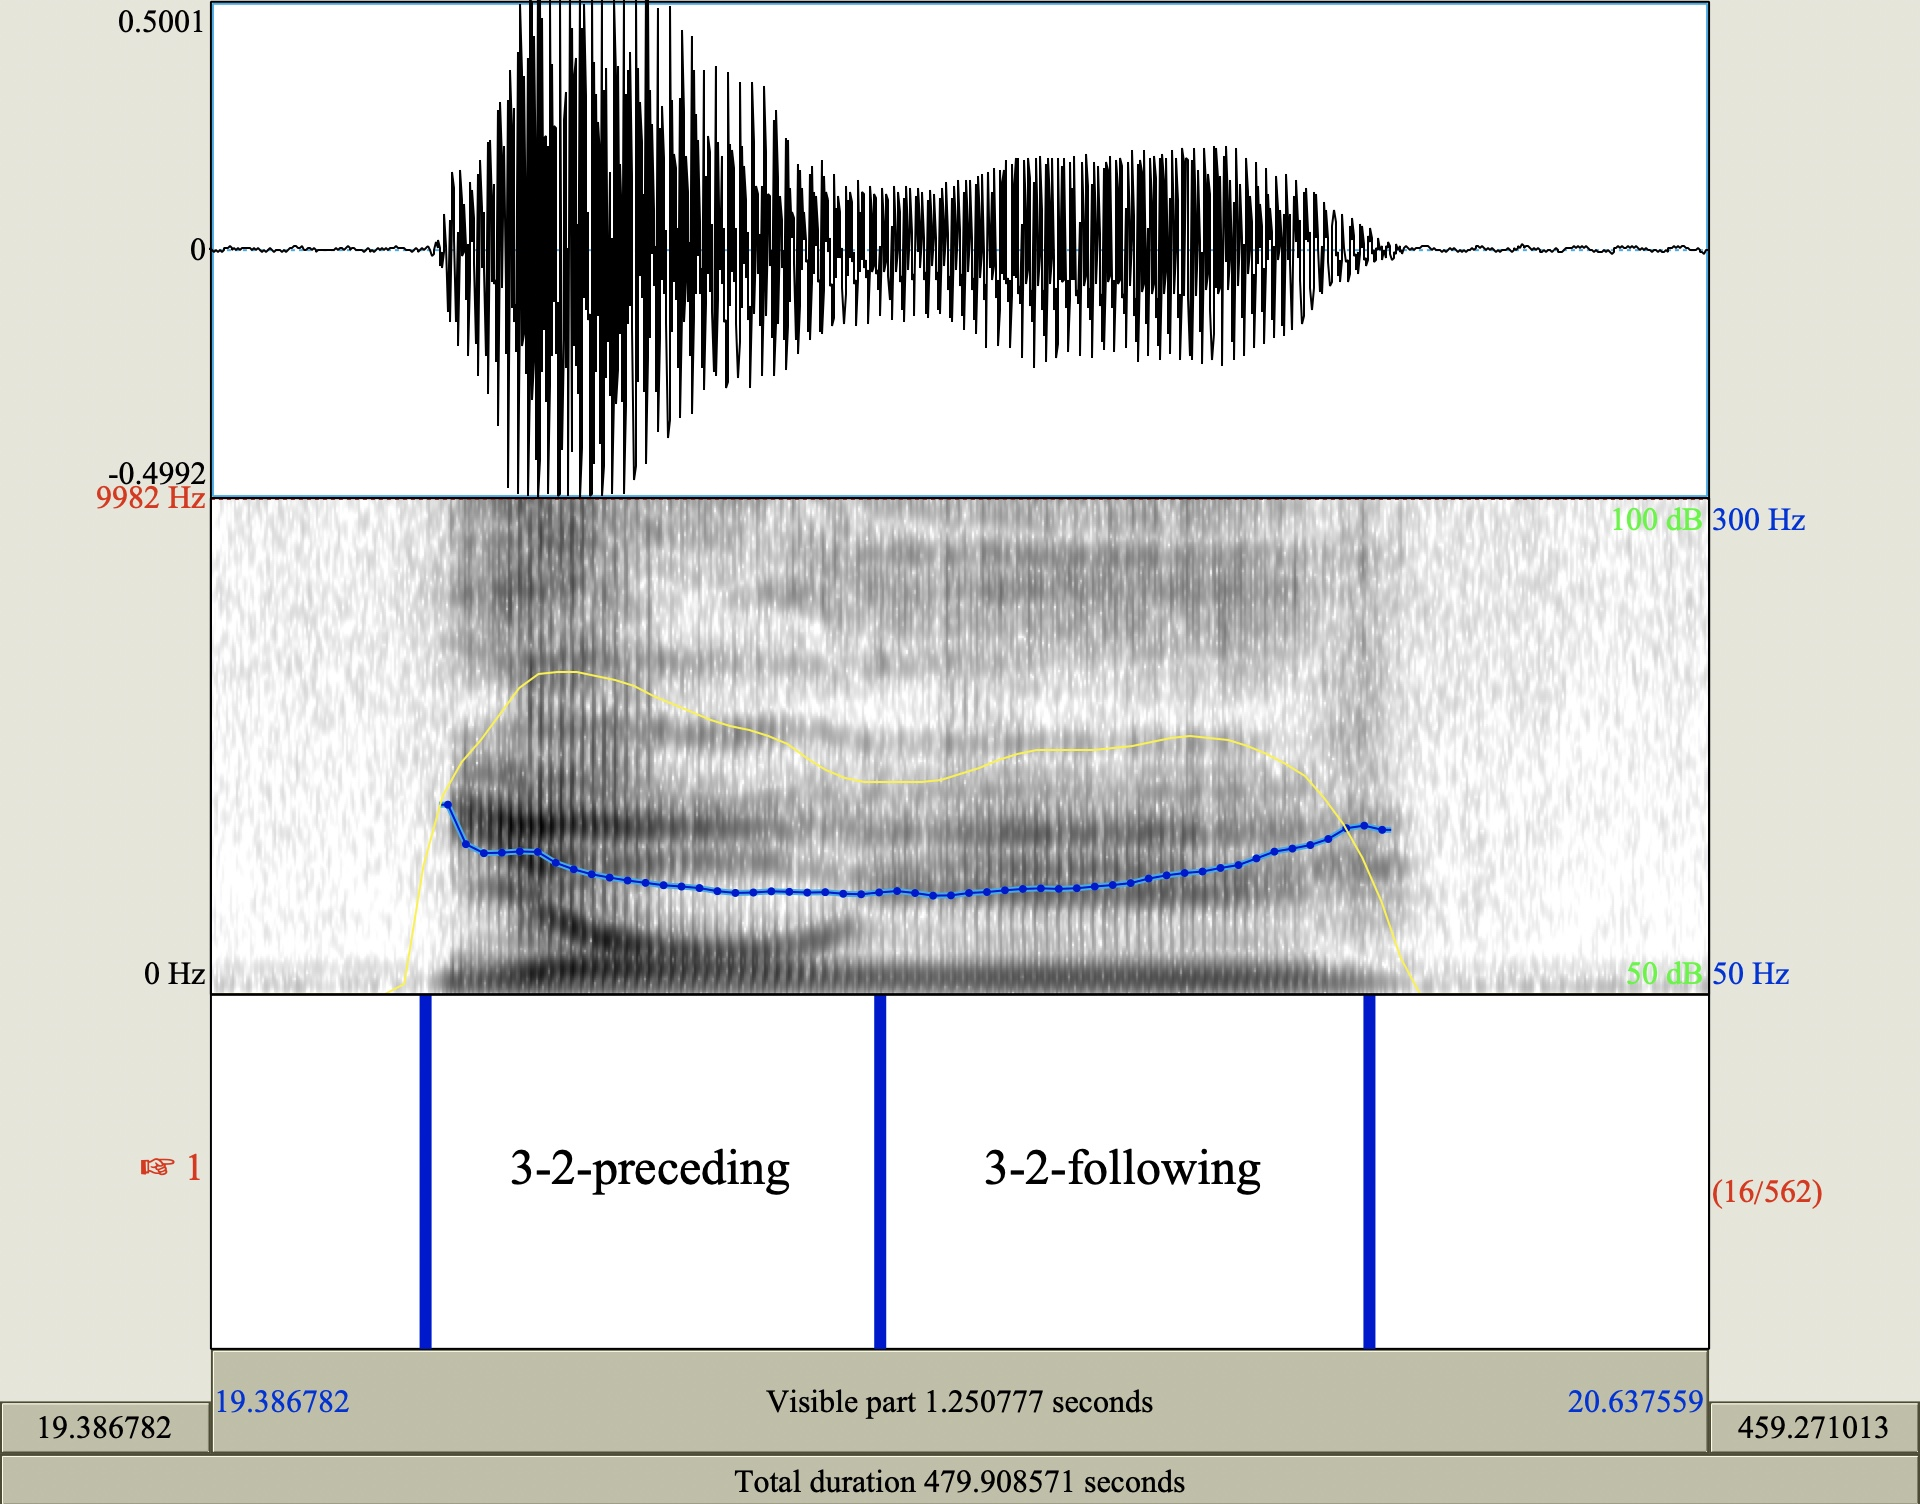
\includegraphics[width=\textwidth]{figures/E1/TextGridExample.jpg}
\caption{Example of TextGrid labeling.}
\label{Figure:TextGridExample}
\end{figure}

\subsubsection{Pitch extraction}\label{section:PitchExtraction}
F0 values were extracted using \textit{Praat}, \textit{Parselmouth} \citep{Jadouletal2018}, and \textit{TextGridTools} \citep{BuschmeierWlodarczak2013} on Python 3.9 \citep{vanRossumDrake2009}. The time step was 0.01s. The pitch ceiling and floor values were determined individually for each tone for each subject. To avoid possible failure to capture the F0 value for every time step, principally due to creaky voicing or extra-low pitch, for each tone production, the F0 values were divided into 11 proportions, missing values in a proportion were ignored, and the mean of the F0 values in each proportion was calculated. If all values in a proportion were missing, this proportion was discarded; if more than 3 of the 11 time points were discarded, this tone production was discarded. After all F0 values were extracted, they were converted to z-transformed semitones to make cross-subject comparison. 4.13\% of Taiwan Mandarin and 11.08\% of Taiwan Southern Min tokens were discarded.

\subsection{Analyses}
\subsubsection{Pitch contour comparison}
For visualization and direct observation, F0 data were fitted through generalized additive mixed models (GAMMs; \citealp{Wieling2018}) with R Core \citep{RCoreTeam2019}’s \textit{lme4} package \citep{Batesetal2015}.

\subsubsection{Tonal coarticulation}
To quantify the magnitude of tonal coarticulation, the pitch onsets and offsets were first calculated. These were determined as the F0 means of the first and last 9.0\% (i.e. the first and last of the 11 time points mentioned in Section \ref{section:PitchExtraction}) of each tone production, with missing values ignored. Linear mixed-effect models were fitted with R Core \citep{RCoreTeam2019}’s \textit{lme4} package \citep{Batesetal2015}. Several candidate models were compared according to their AIC scores. The chosen models had as the fixed effects the values of preceding offsets (in the case of carry-over coarticulation)/following onsets (in the case of anticipatory coarticulation, shown as \textit{x} in the code), language (Taiwan Mandarin vs. Taiwan Southern Min), and tones. Participants were taken as random inetrcepts, with a random slope of \textit{x} on each of level of \textit{participant}. The formula is shown below\footnote{In the case of carry-over coarticulation, \textit{y} is the values of the following onsets; in the case of anticipatory coarticulation, it stands for the values of the preceding offsets.}:

\begin{lstlisting}
    model <- lmer(y ~ x*language*tone + (x|participant))
\end{lstlisting}

In order to compare the magnitudes of carry-over and anticipatory effects within each of the two languages, other two models were fitted, with the fixed effects being the onset/offset values, positions (carry-over vs. anticipatory), and tones, and the same random effects as in the previous models.

\begin{lstlisting}
    model <- lmer(y ~ x*position*tone + (x|participant))
\end{lstlisting}

In this study, significant results (p<.05) were taken as indicator of existence of tonal coarticulation; positive coefficients were taken as indicator of assimilatory effects, and negative ones indicator of dissimilatory effects.

\section{Experiment 2}\label{section:Experiment2}
Experiment 2 measures the perceptual compensation for tonal coarticulation in Taiwan Mandarin and Taiwan Southern Min. Following the design of \cite{Zhangetal2022}, a continuum from low-level tone to falling tone preceded by tones of different pitch levels of offsets were synthesized into disyllabic stimuli, and subjects were asked to judge whether they heard a low-level tone or a falling tone. If perceptual compensation was at work, different pitch levels of preceding offsets should render different thresholds of low-level tone/falling tone judgement.

This experiment was divided into a Mandarin version and a Southern Min version.

\subsection{Participants}
All 43 participants participated in this experiment. The monolingual group did the Mandarin version. The bilingual group did both the Southern Min and Mandarin versions.

\subsection{Stimuli}
\subsubsection{Word selection}
3 Pairs of Taiwan Mandarin disyllabic words and 4 pairs of Taiwan Southern Min words were chosen for each of the two versions. These pairs were minimal pairs that differed only in the tones of the second syllables. Within each pair, the first syllables were the same and served as the primes, while the second syllables were the targets, and were a low-level tone and a falling tone, respectively. In this experiment, all tones in both languages that were suitable to serve as the primes were accounted for. In Taiwan Mandarin version, there were 3 pairs of words, with the primes (i.e., first syllables) of each pair being 55 (T1), 35 (T2) and 51 (T4), respectively, and the low-level tone being 21 (T3) and falling tone 51 (T4). The pairs were therefore T1+T3/T4, T2+T3/T4, T4+T3/T4. T3 as the primes were excluded due to tone sandhi. For Taiwan Southern Min version, 4 pairs of words were chosen, with the first syllables of each pair being 33 (T5'), 55 (T2'), 51 (T3'), and 21 (T7'), and the low-level tone being 21 (T3), and falling tone 51 (T2). The checked tones, 32 (T4'), and 54 (T8'), were excluded due to their inherently shorter durations. T1' was ignored since its value was the same as T5' (33) in the dialect we chose (the Southern dialect). 35 (T2') was also excluded since only the Quan dialect applies this sandhi rule. The pairs were thus T5'+T3/T2, T2'+T3/T2, T3'+T3/T2, T7'+T3/T2. See Appendix \ref{Appendix:StimuliforExperiment2} for the words used.

\subsubsection{Stimuli recording}
The words were produced by one male native speaker (25 y.o.) of Taiwan Mandarin and one male native speaker of Taiwan Southern Min\footnote{He was also native speaker of Taiwan Mandarin.} (24 y.o.). The same apparatus used in Experiment 1 was used.

\subsubsection{Stimuli syntheses}
Following \cite{Zhangetal2022}, the stimuli were synthesized into continua where the pitch contours of the first syllables were made sure to be the same, and the pitch contours of the second syllables went from a low-level contour to a falling contour. The F0 values for the contours of the primes were converted from the five-level tone sacles with the equation of \cite{FonChiang1999}:
\[scale = \dfrac{1}{2}(39.86\times \log (\dfrac{f_{i}}{f_{min}})) + 1\] In this study, the $f_{min}$ was set at 100 Hz. This was approximately the natural pitch low point of the two speakers. The converted F0 values from scale 1 to 5 were: 100, 112.25, 125.99, 141.43, and 158.75 Hz. The starting F0 values of the targets were divided into 10 levels on Bark's scale. The minimum was 0.9 and the maximum 1.9 on Bark's scale, with the step being 0.1. The end point was the minimum (0.9). The F0 values of this continuum in Hz were: 90.34, 101.59, 112.88, 124.2, 135.57, 146.99, 158.45, 169.97, 181.55, 193.19. The mean intensities of all syllables were scaled to be the same, and the durations of all syllables were 0.3 s. Illustrations of the synthesized pitch contours are given in Figure \ref{Figure:SynthesizedToneContours}.

\begin{figure}[h]
\centering
\includegraphics[scale=.3, trim={0 8.5cm 0 0}]{figures/E2/SynthesizedToneContours.png}
\caption{Illustrations of synthesized pitch contours (top: Taiwan Mandarin version; bottom: Taiwan Southern Min version).}
\label{Figure:SynthesizedToneContours}
\end{figure}

The audio data of the original disyllabic words produced by the two speakers were first exercised into separate syllables. The syllables's F0 values were then synthesized to match those presented in Figure \ref{Figure:SynthesizedToneContours}. The durations and intensities of the syllables were then adjusted using \textit{FFmpeg} \citep{Tomar2006}. The separate syllables were then concatenated back into a single audio file with Python's \textit{wave} package.

For Taiwan Mandarin version, there were a total of 150 stimuli (10 levels$\times$3 tones$\times$5 repetitions). For Taiwan Southern Min version, there were a total of 200 stimuli (10 levels$\times$4 tones$\times$5 repetitions).

\subsection{Procedure}
The experiment was created with PsychoPy \citep{Peirce2019} and Javascript \citep{Flanagan2006}, and hosted on Pavlovia (\url{https://pavlovia.org}). For each trial, the subject would first see a cross, then see an ear picture, and hear the stimulus at the same time, and then the two corresponding minimal pairs would appear. The subject was required to click on the one he/she thought he/she heard. For Taiwan Mandarin version, the words were presented in traditional Chinese; for Taiwan Southern Min version, both the traditional Chinese characters and their romanizations were presented, where word 1 was the one that ended with the low-level tone, and word 2 the one with the falling tone. An illustration of a single trial is given in figure  \ref{Figure:Experiment2Procedure}. The stimuli were pseudo-randomly shuffled so no words in the same pair would be used in two consecutive trials. Before the formal trials started, the subject was given 4 practice trials. The Taiwan Mandarin version took about 7 minutes and the Taiwan Southern Min version about 10 minutes. To ensure the subjects were familiar with the stimuli, they were presented slides with the the orthographies of the stimuli, illustrative pictures, and the stimuli's meanings on them. One of the slides is shown in Figure \ref{Figure:Experiment2SlideExample}. The participants were also told this and the following experiment (Experiment 3) were not a listening comprehension test, and that they should be relaxed and follow their instincts.

\begin{figure}[h]
\centering

\includegraphics[width=.7\textwidth]{figures/E2/SlideExample.jpg}
\caption{Example of the slides used to familiarize the subjects with the stimuli.}
\label{Figure:Experiment2SlideExample}
\end{figure}


\begin{figure}[h]
\centering
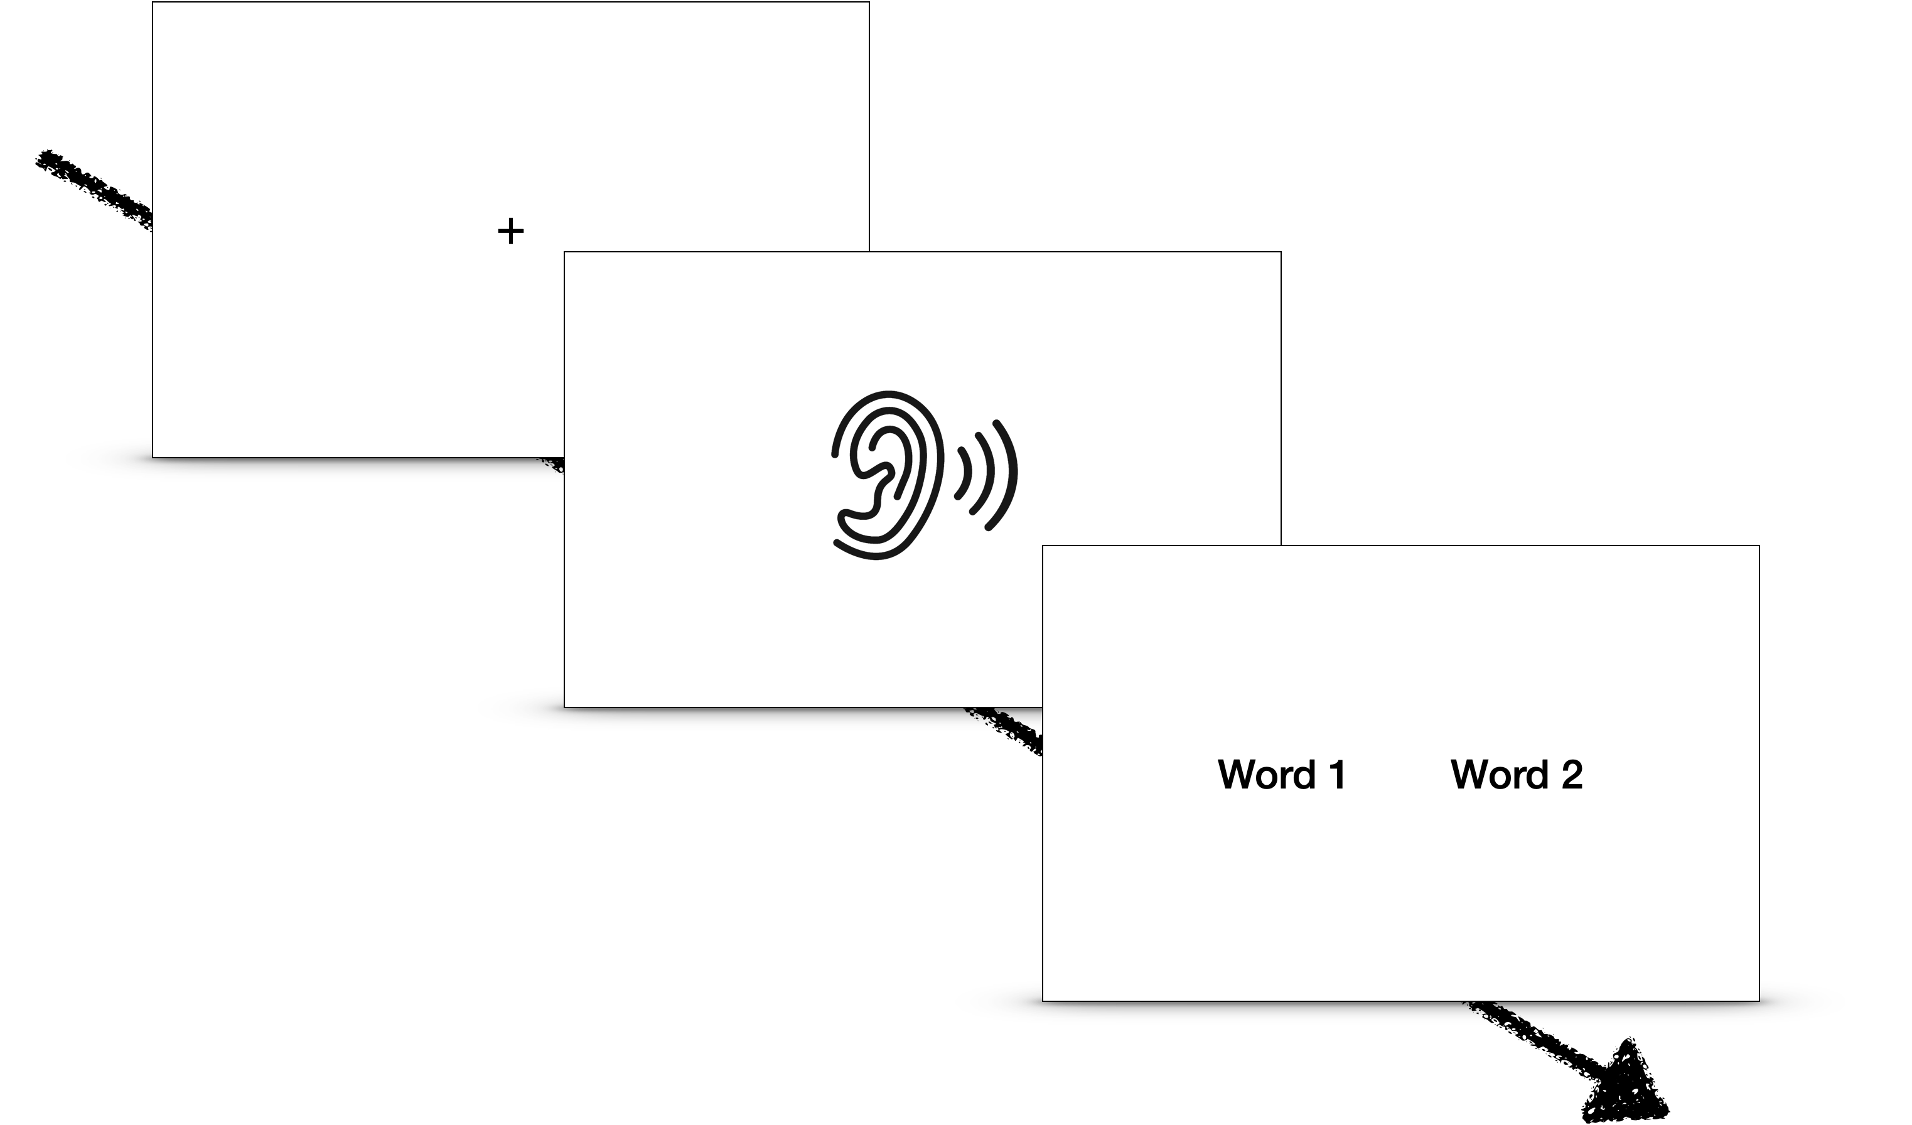
\includegraphics[width=.7\textwidth]{figures/E2/Procedure.png}
\caption{Procedure of Experiment 2.}
\label{Figure:Experiment2Procedure}
\end{figure}

\subsection{Analyses}
The responses of the subjects were calculated as percentages of falling tone responses (cf. Figure \ref{Figure:E2RawExample}), and then fitted through logistic regression models. A 25\% and a 75\% thresholds were set. Mean differences between the smallest and the largest crossing points on the two thresholds were taken as indicators of the magnitudes of perceptual compensation for tonal coarticulation. An illustration of such calculation is provided in Figure \ref{Figure:E2ProcessedExample}.

\begin{figure}[h]
\centering
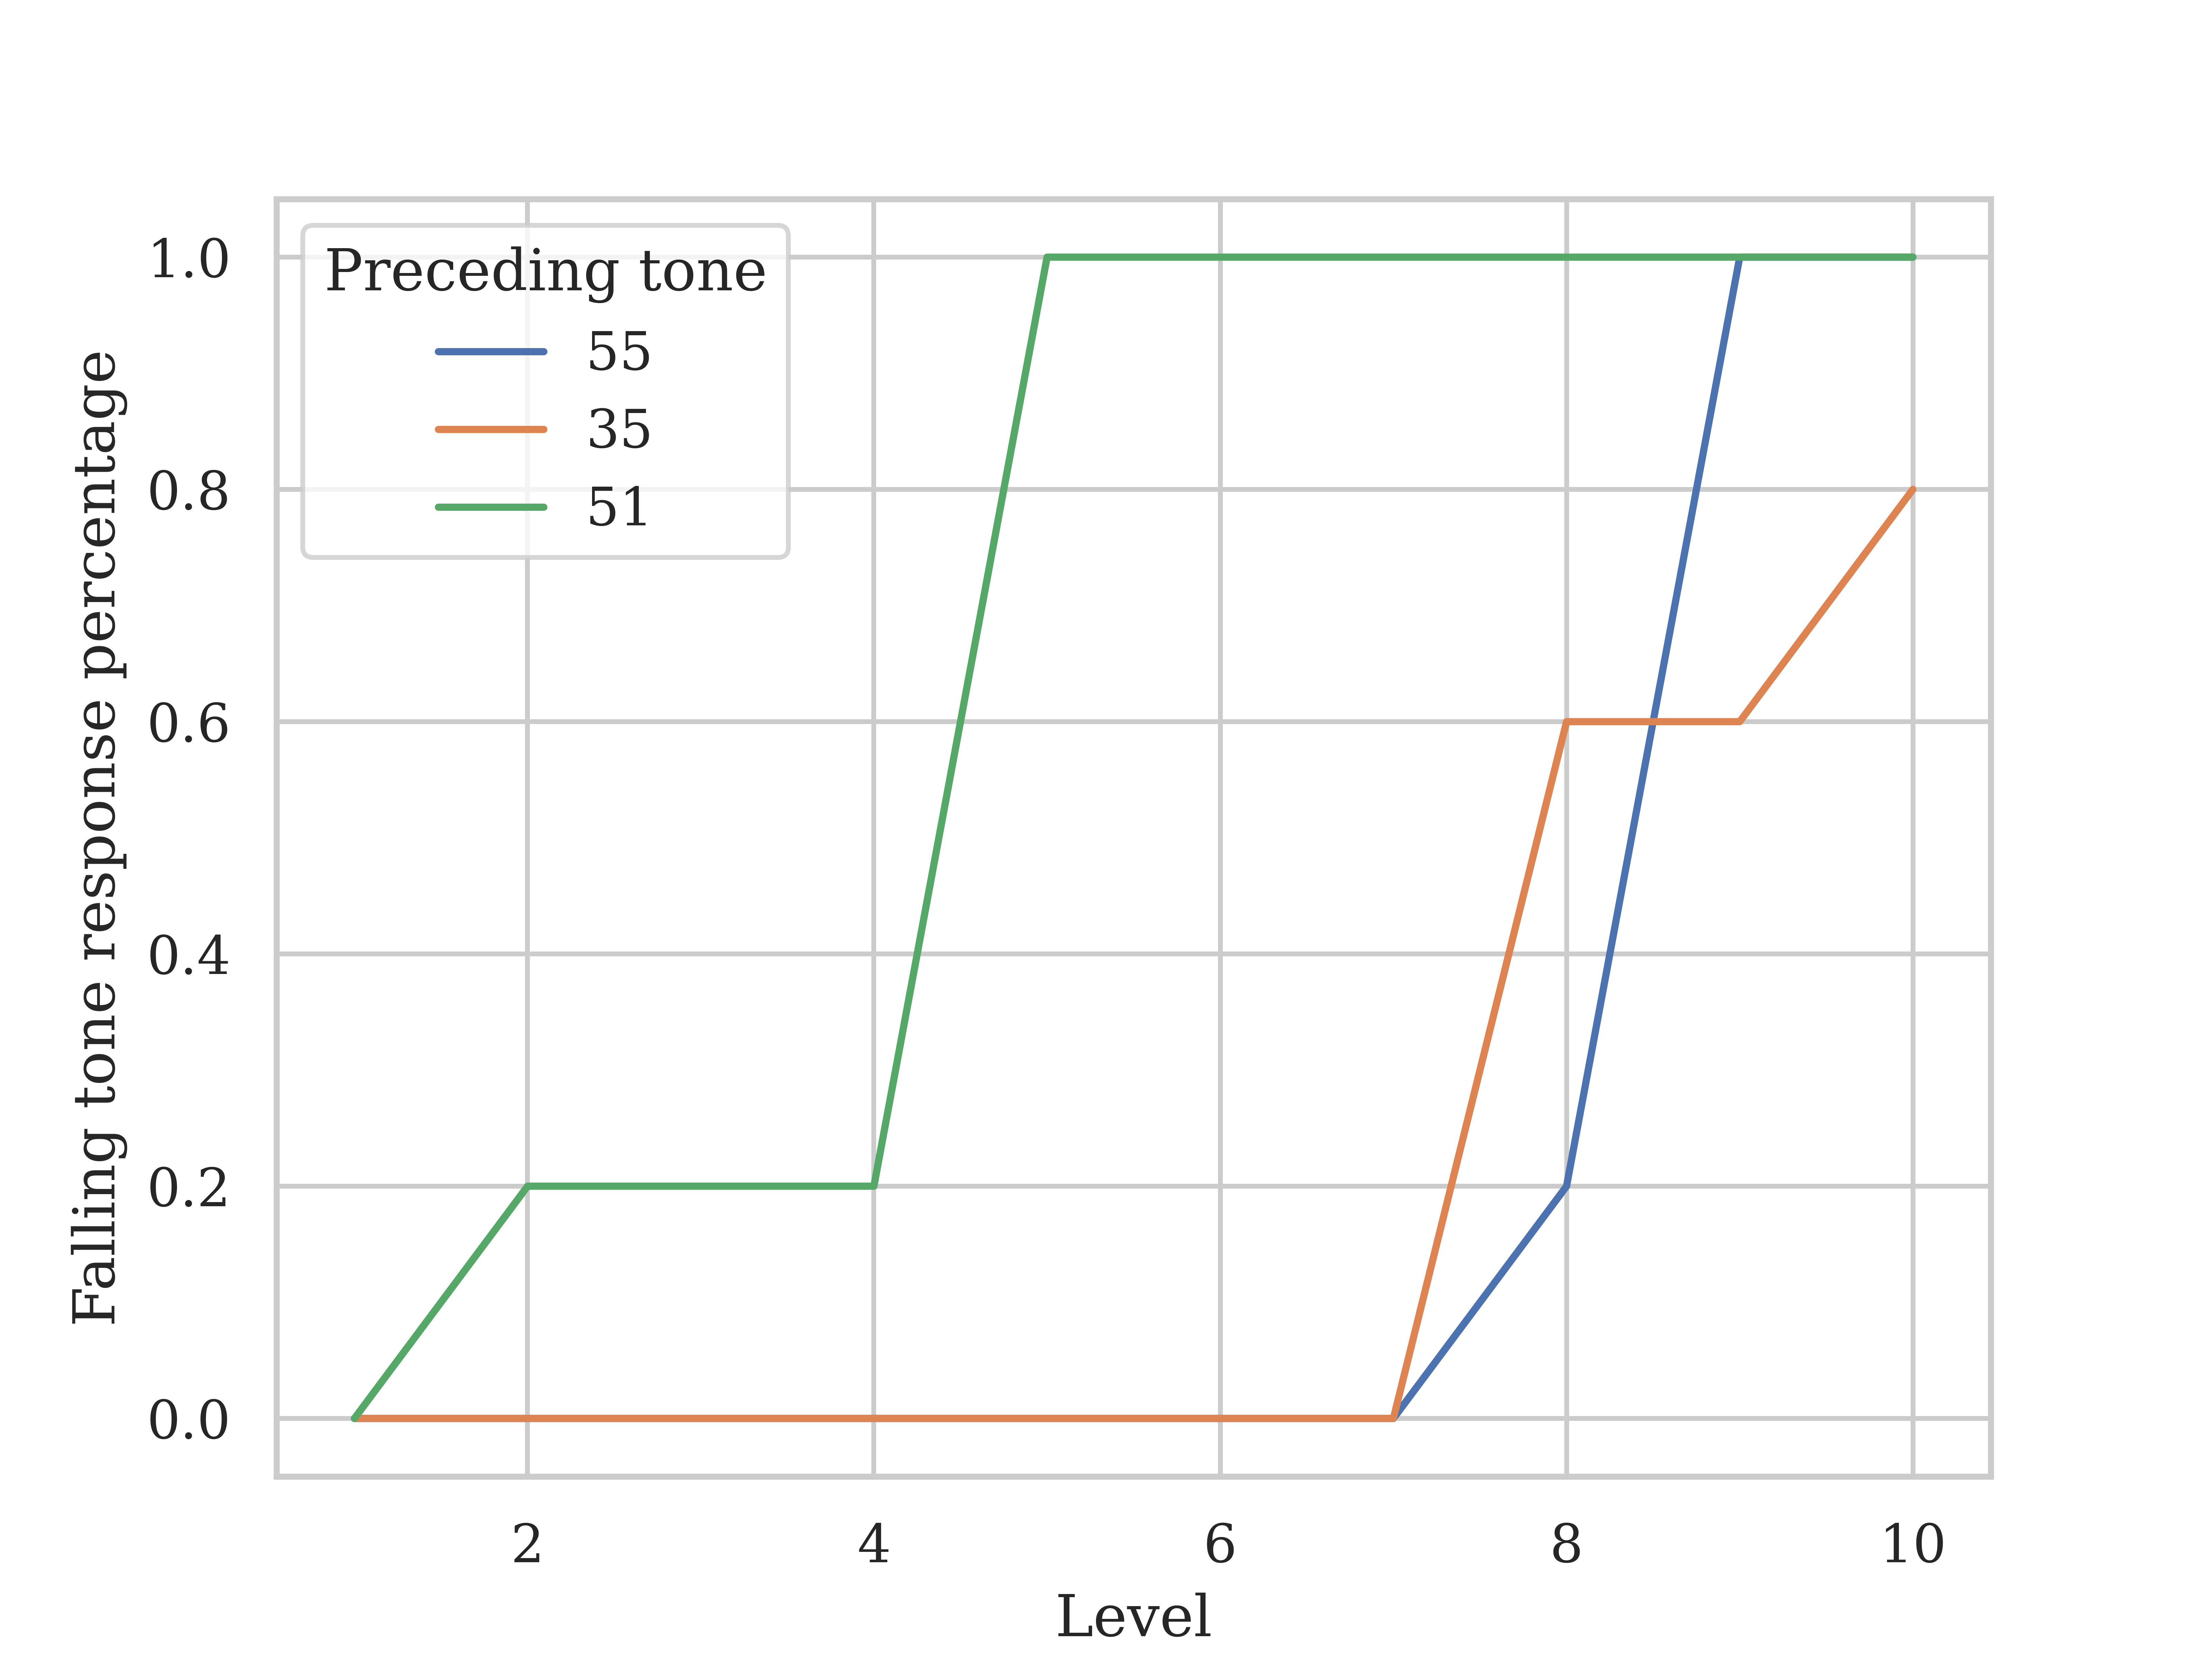
\includegraphics[width=\textwidth]{figures/E2/RawExample.png}
\caption{Example of percentages of falling tone responses (data of P1).}
\label{Figure:E2RawExample}
\end{figure}

\begin{figure}[h]
\centering
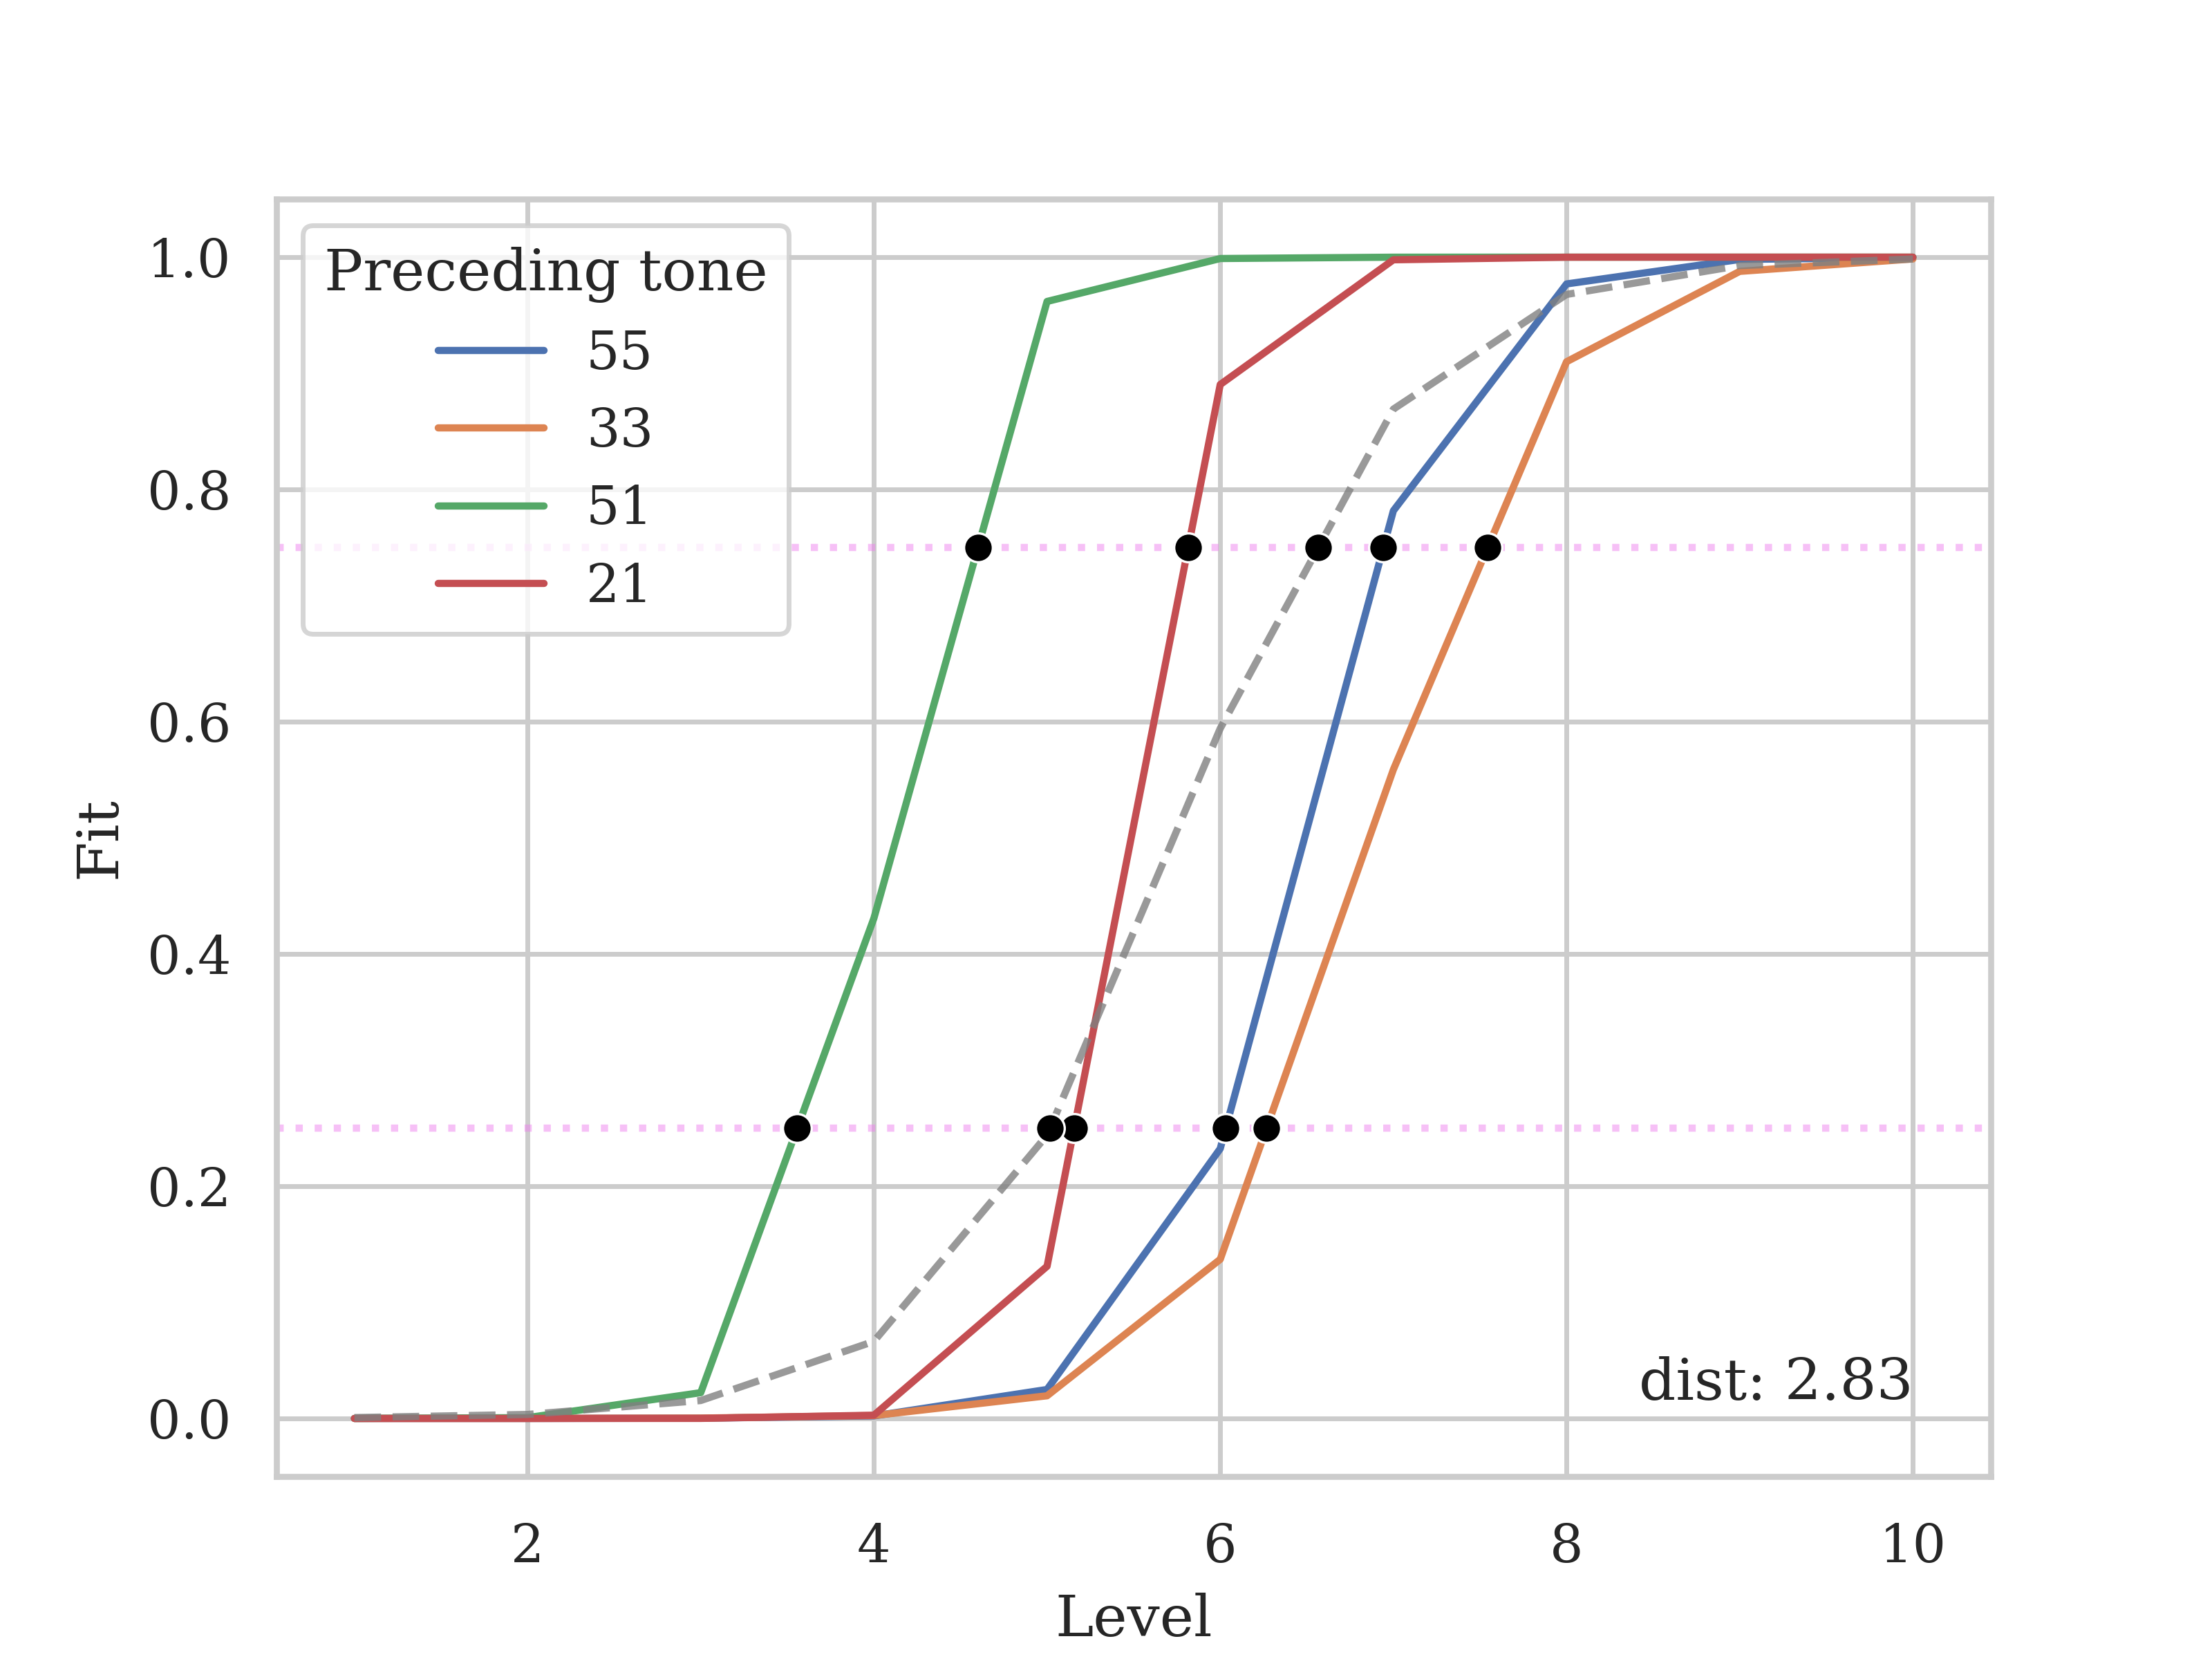
\includegraphics[width=\textwidth]{figures/E2/ProcessedExample.png}
\caption{Example of mean distance calculation (data of P1).}
\label{Figure:E2ProcessedExample}
\end{figure}

\section{Experiment 3}\label{section:Experiment3}
To explore the relation between perceptual compensation for tonal coarticulation and strictness of tone boundaries, Experiment 3 was conducted to see whether there exists differences between the acceptance ranges of falling and low-level tones in Taiwan Mandarin speakers and Taiwan Southern Min speakers.

To measure the subjects' strictness of tone boundaries, subjects listened to a continuum of falling and low-level tones after the high-level (55) tone (T1 in Taiwan Mandarin; T2' in Taiwan Southern Min), and were asked to judge whether what they heard were good tokens of the intended target tones.

This experiment was also divided into the Mandarin and Southern Min versions.

\subsection{Participants}
The same subjects in Experiments 2 participated in this experiment. The monolingual group did the Mandarin version; the bilingual group did both the Mandarin and Southern Min versions.

\subsection{Stimuli}
\subsubsection{Word selection} In each version, 10 disyllabic words were used. All of their first syllables were the high-level tone. 5 of them had as their second syllables the falling tone, and 5 of them the low-level tone. There were therefore 2 groups of stimuli: 55 "(T1 in Taiwan Mandarin; T2' in Taiwan Southern Min)+51 (T4 in Taiwan Mandarin; T2 in Taiwan Southern Min) and 55+21 (T3 in Taiwan Mandarin and Taiwan Southern Min). The words were made sure to have no minimal pair counterparts; that is, the words in the 55+21 group would be non-words if the second syllables were changed into a falling tone, and vice versa. See Appendix \ref{Appendix:StimuliforExperiment3} for the words used.

\subsubsection{Stimuli recording and synthesis}
Stimuli were produced by the same speakers in Experiment 2, and recorded and synthesized the same way as in Experiment 2. Since the words, unlike those in Experiment 2, were not minimal pairs, a 55+21 stimulus would be less like a word as the level went up on the continuum, and vice versa for a 55+51 stimulus.

For each level of the 55+21 and 55+51 groups, there were 10 repetitions. For each repetition, one of the five words were randomly chosen. There were therefore a total of 200 (2 groups$\times$10 levels$\times$10 repetitions) stimuli.

\subsection{Procedure}
This experiment was conducted after Experiment 2, after a minimal 1 minute break. The procedure and presentation were the same as those of Experiment 2, except that only one word was presented in the middle of the screen, with two buttons, a cross and a circle, underneath. The subject was asked to decide whether he/she thought it was a correct production of the word they saw. Figure \ref{Figure:Experiment3Procedure} illustrates such process. Participants were familiarized with the stimuli the same way as in Experiment 2.

\begin{figure}[h]
\centering
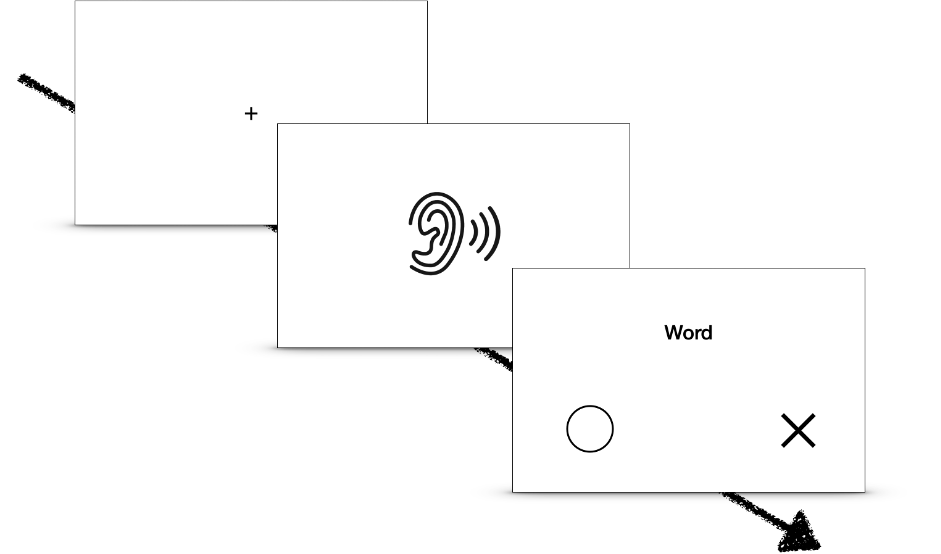
\includegraphics[width=.7\textwidth]{figures/E3/Procedure.png}
\caption{Procedure of Experiment 3.}
\label{Figure:Experiment3Procedure}
\end{figure}

\subsection{Analyses}
The subjects' responses were calculated as percentages and taken as acceptance rates of each of the 10 levels. These were then fitted through logistic regression models. The maximum slopes of each regression lines were taken as indicators of how strict/tolerant the subjects' tonal acceptances were. A steep slope would indicate that the subject was very strict on how the pitch values/contours of a given tone should be, and a flatter slope would suggest the subject had a wider acceptance range for the pitch of a given tone. An illustration is provided in Figure \ref{Figure:E3ProcessedExample}.

\begin{figure}[h]
\centering
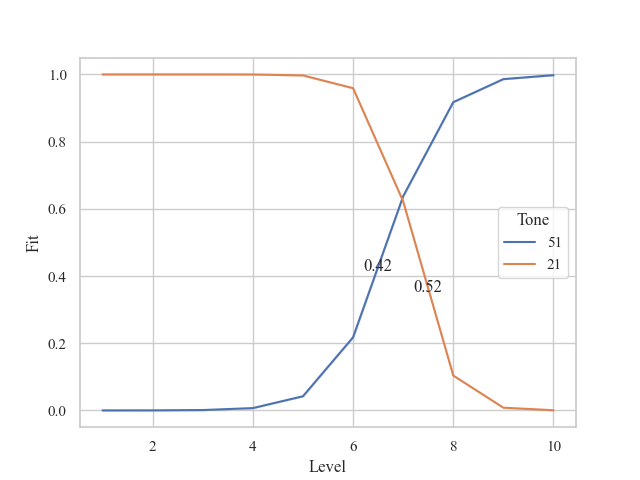
\includegraphics[width=\textwidth]{figures/E3/ProcessedExample.png}
\caption{Example of maximum slope calculation (data of P1).}
\label{Figure:E3ProcessedExample}
\end{figure}
